\chapter{Background}
\label{ch:preliminaries}

In this chapter, we outline the relevant terminologies and the theoretical  preliminaries that is essential for better understanding of this essay.
This chapter is sectioned into 3 parts.
Section \ref{sec:bck_rdf_model} describes essential concepts of RDF as a modeling language and its main serialization formats. 
In Section \ref{sec:bck_parser}, parsing techniques and methods to detect and recover syntax errors are discussed. Finally, Section \ref{sec:bck_ANTLR} presents an overview of ANTLR parser generator which is used to automatically generate the internal parser of RDF-Doctor.


\section{The Resource Definition Framework}
\label{sec:bck_rdf_model}

The "Semantic Web" \cite{W3C:SemanticWebTerm:Online} term  has appeared during the transformation process of web development from "Web of documents" to "Web of data", similar to those data found in databases. 
W3C defines it as "the Web of linked data". {Figure \ref{Fig:semanticWebStack}} describes the Semantic Web Stack, proposed by W3C. 
It can be seen that it contains several technologies to enable the users of creating their own data stores on web, building vocabularies, and enforcing processing rules on such data.   

Subsequently, in order to make data more and more machine-readable and interchangeable between various applications, RDF model \cite{W3C:RDF-Primer:Online} has been proposed.  To elaborate, RDF model plays a fundamental role of data exchange in the layered Semantic Web Stack and links the high-level semantic web tools with low-level ones, as exhibited in {Figure \ref{Fig:semanticWebStack}}. 
	\begin{figure}[ht]
	\begin{center}
	\setlength\belowcaptionskip{-7mm}
		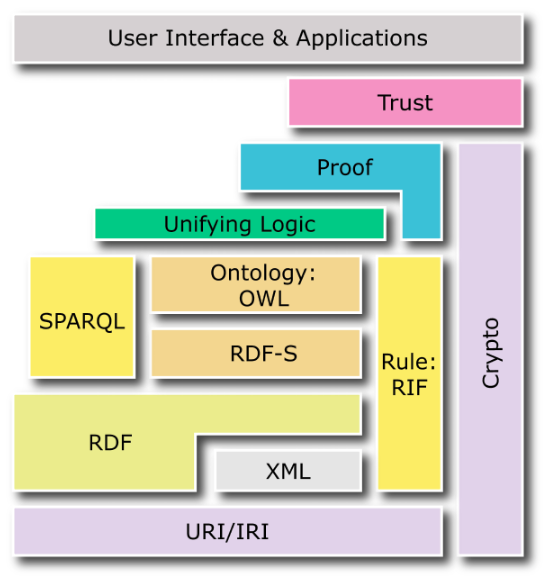
\includegraphics[scale=0.5,angle=0]{images/semanticWebStack}
		\caption{\textbf{The Semantic Web Stack \cite{W3C:SemanticStack:Online}.} RDF Model links  high-level semantic web tools with low-level ones and works as a bridge to enable data exchange between various applications}
		\label{Fig:semanticWebStack}
	\end{center}
\end{figure}
\par
Also, {Figure \ref{Fig:rdfModel}}(a) presents how data are engineered in RDF Model in triples. A triple is defined by 3 main components: a subject, a predicate, and an object. It has a common similarity of a basic structure of a simple sentence in a natural language which consists of a subject, a verb, and  an object. As the verb in natural languages shows a relation and a connection between the other two entities, in the same way in RDF Model, the predicate connects both subject and object in a certain property. 

\subsection{Simple Example of RDF Model}

To make it more clear, a simple example of RDF Modeling is giving in Figure \ref{Fig:rdfModel}(b). A fact to express that "German has the river Rhein", \textbf{Ex:Germany} is a subject, \textbf{Ex:hasRiver} is a predicate, and \textbf{"Rhein"} is an object. The first two terms are Uniform Resource Identifiers (URIs) where \textbf{Ex:} is a declared prefix label in RDF file to refer to an URI path and the following part \textbf{Germany} is an extension of the path. The last value \textbf{"Rhein"} is a literal or a string. What is given is a simple example of RDF Model to show its fundamental structure, but, in the meanwhile, more examples can be viewed at \cite{W3C:RDF-Primer:Online}.

\begin{figure}[ht]
	\begin{center}
		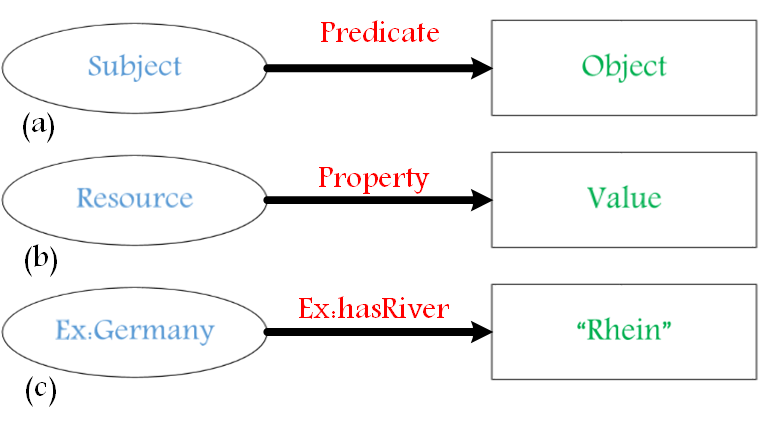
\includegraphics[scale=0.4,angle=0]{images/RDF-Model}
		\setlength\belowcaptionskip{-5mm}
		\caption{\textbf{ Structure of RDF with Example.} A triple is a major component in RDF Model which has a form of Subject-Predicate-Object, as shown by (a), while an example of a triple is presented by (b).}
		\label{Fig:rdfModel}
	\end{center}
\end{figure}
RDF data can be represented in a couple of serialization formats, as was mentioned in Chapter \ref{ch:introduction}. Since their syntax used as use cases to be parsed with RDF-Doctor , In the next two subsection, N-Triples and Turtle are discussed. 
\subsection{N-Triple Serialization}
N-Triples \cite{W3C:Ntriples:Online}

\subsection{Turtle Serialization}
 Terse RDF Triple Language (Turtle) \cite{W3C:Turtle:Online} is one of RDF serialization formats, it uses triples for data representation. A triple has Subject-Predicate-Object form, it  has a similarity with some of natural languages where a simple sentence consists of a subject, a verb, and an object. In order to understand the syntax of Turtle, some terms  relevant to such syntax are discussed as follows.

\begin{itemize}
    \item \textbf{URI\footnote{https://tools.ietf.org/html/rfc3986
:}} it refers to a Uniform Resource Identifier, used to point to a web resource, not only a web page, as a Uniform Resource Locator (URL) do. it has two forms: a normal form (similar to URL in-between brackets) and a short form (can be referred as \textbf{Prefixed-Name})

    \item \textbf{Blank Node:}
    \item \textbf{Prefix:} it is a  short-cut way to replace long URIs with abbreviated ones. essentially, it contains a Prefix-Label.
        \item \textbf{Prefixed-Name:}
        \item \textbf{Prefixed-Label:}
        \item \textbf{Prefixed-URI:}  
  
    \item \textbf{Literal:} a string or a number
\end{itemize} 

The main players in Turtle syntax are prefixes and triples. Prefixes are used to make Turtle a user-friendly language and to reduce the redundancy of repeating some values. A prefix starts with a keyword \textbf{@Prefix} and \textbf{PREFIX} can be also used, followed by \textbf{Prefix\_label} such as "rdf", followed by a \textbf{colon}, next \textbf{Prefix\_URI} \textbf{in-between  2 Brackets} for that prefix, and a \textbf{dot} ends the prefix line. 


Similarly, a base URI can be declare similar to the prefix syntax, with replacing @prefix with \textbf{@base} or \textbf{BASE} 


Next, in points, the syntax of Turtle is described:
\begin{itemize}
    \item Each directive or triple ends with a dot.
    \item Subject can be either a blank node, or URI. 
    \item Predicate is only URI.
     \item Object can be either an URI, a Literal or an blank node.


\end{itemize} 

\begin{figure}[ht]
	\begin{center}
		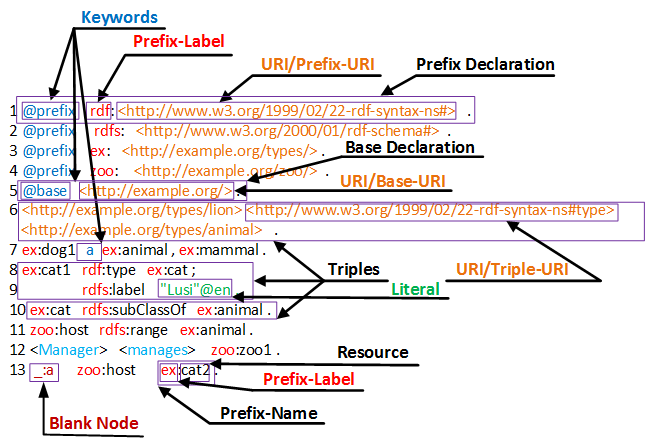
\includegraphics[scale=0.8,angle=0]{images/TurtleStructure.png}
		\setlength\belowcaptionskip{-5mm}
		\caption{\textbf{ Structure of Turtle with Example.} Multiple terms draw the syntax of Turtle, they are shown with one or more matched patterns}
		\label{Fig:TurtleStructure}
	\end{center}
\end{figure}
\section{Parsing and Error Recovery}
\label{sec:bck_parser}
This subsection defines "Parsing" and "Grammar" terms, shows the role of the parser in the compiler, discusses types of parser developments, and finally, it lists the methodologies of error recovery in parsers. 
\subsection{Parsing and Grammar Definitions}
It is of great benefit to shed a light on parsing term to understand later the approach of this study. In \cite{parsingGuide2017}, Gabriele Tomassetti has defined \textbf{Parsing} by:{\it  \textbf{``The analysis of an input to organize the data according to the rule of a grammar''}}. It can be intelligibly recognized that parsing deals with some input data and tries to analyses it based on a given grammar. let's have a look on the definition of grammar based on  \cite{parsingGuide2017},as well. \textbf{Grammar} is 
{\it \textbf{``A formal grammar is a set of rules that describes syntactically a language''}}. In the definition, rules are the significant part of the grammar to define a syntax of a language.  
\subsection{Parser Role in Compilers}
The parser is an essential element in  compilers. {Figure \ref{Fig:parserPosition}} draws the role of the parser in a compiler. The first component "Lexical Analyzer" receives the input data, then produces tokens for  the "Parser" component. Parser constructs a parse tree based on its grammar rules and gets the next token until it consumes all the tokens. The parse tree as an output of the parser is delivered to the next phases of the compiler. If any errors are found, lexical errors can be generated by Lexical Analyzer and Parser is the producer of both syntax and semantic errors. 
%TODO{add the ref or change the image}

\begin{figure}[ht]
	\begin{center}	\setlength\belowcaptionskip{-5mm}
	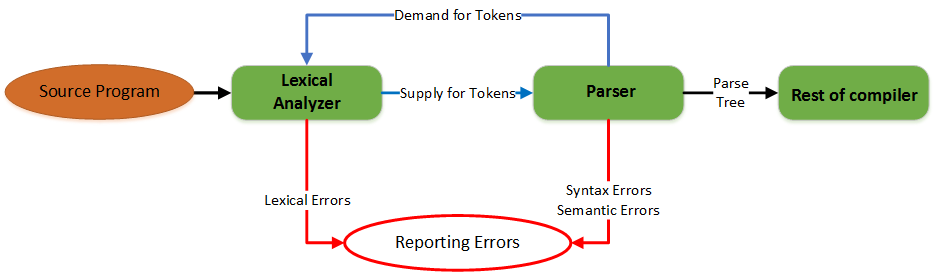
\includegraphics[scale=0.55,angle=0]{images/ParserRole}
	\caption{\textbf{Role of Parser in compilers}. a parsing process in a compiler has 2 main elements: a Lexical analyzer and a parser, the former supplies tokens to the latter, once it has enough tokens to be parsed, it parse them, and asks the former to continue of the tokens supplement, the former generates lexical errors and the latter produces syntax ans semantic errors when parsing a source program, the parse tree is the output of the latter }
		\label{Fig:parserPosition}
	\end{center}
\end{figure}
\subsection{Parser Developments}
In order to build a parser, there are two available options, either by starting  to code own parser  or getting an off-the-shelf automatic parser generator tool that automatically creates the parser source code from a grammar file. In the following, both approaches are outlined:

\textbf{1) Writing a parser source code from scratch:} it is to write own parser source code from A to Z, including the lexical analyzer and the parser classes. On the one hand, this way gives more flexibility in handling several issues, triggered when dealing with certain token patterns, such as special characters and escape sequences. On the other hand, it consumes much time and requires a large amounts of  effort.

\textbf{2) Generating a parser source code using automatic parser generators:} a parser generator outputs the desired parser source code. Predominately, such tools can be used to do a specific parsing task, but again, a grammar identifying the  demand syntax is required as an input for those tools. To elaborate, the competitive advantage here is the less needed time and effort to build a parser, However, the flexibility is reduced to what features and classes provided by those tools, otherwise, such flexibility can be  optimized by adding new classes and modules to more features, for example to parse a large file, frequently, an "full memory space" error is fired, by adding a class that divides the large file into chunks to be sequentially parsed, can solved this issue and add such new feature.  

\subsection{Error Recovery Methodologies in Parsers}
In parsers, the error recovery techniques specify the parser behavior, once an error is detected.  Aho et al \cite{Aho:2006}, the researchers in the compiler field    have outlined such techniques as follows:
\begin{itemize}
	\item \textbf{Panic-Mode Recovery}: once an error has been discovered, the parser ignores and skips next input symbols, one by one till a recognized set of tokens is detected. In spite of its discarding of huge number of input symbols without checking them for further error detection, it is considered a simple parsing mode and do not fall in an infinite loop while other modes may do.
	\item \textbf{Phrase-Level Recovery}: to continue the parsing process, the parser performs local correction. A typical local correction in RDF data, for example, is to insert a missing dot or delete extraneous dots.
	\item \textbf{Error Productions}: by expecting  common and well-known errors, production rules can be inserted into the grammar. Then, the generated parser is well-informed about such errors. Error detection and error recovery can be easily done in this case where error details are in our hand, such as the error location, the exact type of error, etc. Equally important a customized and meaningful error message for the identified error can be provided as well. 
	\item \textbf{Global Correction}: conventionally, the parser tries to reduce as much as possible number of change operations (such as, insertion, deletion and modification operations), when dealing with an incorrect input token to reduce globally total cost of error correction. To make it more clear, let's assume an incorrect input statement X is giving in grammar G, the parser constructs a closest error-free parse tree of statement Y to replace statement X, such that the changes are small as possible. 
\end{itemize}


\section{ANTLR Parser Generator}
\label{sec:bck_ANTLR}

ANTLR is a handy tool and easy to use for the purpose of generating a specific domain language parser. It is a parser generator to do an automatic generation of a source code of a parser with less time and effort. The core requirement of ANTLR is to define the grammar of the desired language syntax . The grammar contains language rules  drawing the syntax and the semantic of such  language which the parser is built for. 
\par
 As was previously discussed, the compiler has two main subsystems relevant to this study: a lexical analyzer (called also lexer) and a parser. Both lexer and parser are needed to have their rules defined in the grammar file. Lexer rules are those rules which define the terminals, whereas parser rules determine the non-terminals. Another essential point that is the process of parser creation  demonstrated in {Figure \ref{Fig:ANTLR} where the parser program is generated with the help of ANTLR framework. In more details, this parsing process \cite{ANTLR:Tool:Online} is followed, straing from the needed grammar to build the parser, ending with the output of the parse tree at the end of parsing :

\begin{figure}[td]
	\begin{center}
		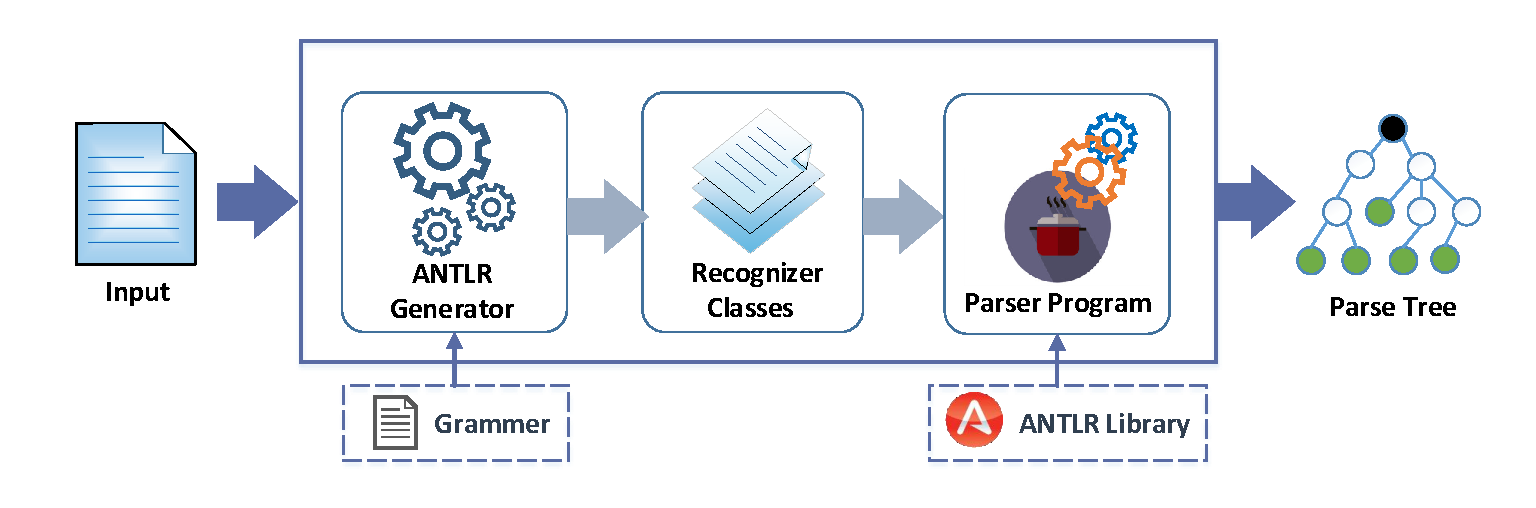
\includegraphics[scale=0.6]{images/ANTLR}
		\caption{\textbf{Parsing process based on ANTLR parser generator\cite{ANTLR:Tool:Online}.} ANTLR parser generator receives the grammar file to generate the classes of the lexer and the parser, when the input text is submitted, the generated classes with using of ANTLR library start the parsing process to generate the parse tree}
		\label{Fig:ANTLR}
	\end{center}
\end{figure}


\begin{enumerate}
		
		\item  {\bf Writing a grammar file:} ordinarily, a grammar called a parsing expression grammar, or PEG is required to build a parser. ANTLR needs a context-free grammar, crafted with the Extended Backus-Naur Form (EBNF). EBNF consists of a sequence of rules. These rules describe the syntax and the semantic of an input which needs to be parsed. Both terminals or non-terminals are types of rule heads. On the one hand, terminals are leaf elements where they have no grammatical structure, e.g., words or numbers. On the other hand, non-terminals have a definite grammatical structure and name, e.g., triples or prefixes. 

		\item {\bf Generation of recognizer target\_based classes by ANTLR:} a significant feature of ANTLR is its capability of generated the auto-generated parser source code for  a variety of the programming languages like \cite{ANTLR:Website:Online}: Java, C\#, Python (2 and 3), JavaScript, Go, C++, and Swift.
		\item {\bf Feeding an input file for parsing:} as an input, ANTLR can parse text documents without additional libraries. Users send their input files for parsing where the parsing process will be achieved based on the crafted grammar in the first step.
		\item {\bf Parsing procedure:} {Figure \ref{Fig:ANTLR} } shows this step as  a phase of cooking . In this step, all materials and ingredients are available. The materials are: 1) the auto-generated parser, and 2) the ANTLR library. The ingredients are one or more text files to be parsed. 
		\item {\bf Delivering of a final report and parse tree as an output:} now, the cake is ready for eating, an output of this process is given to the user containing of a parse tree and a report of collected errors.
	\end{enumerate}











